\chapter{A Programação Linear e as suas Aplicações}

\section{Introdução}
Na pesquisa operacional, a programação linear é uma das técnicas mais utilizadas em problemas de otimização. Os problemas de programação linear geralmente buscam a distribuição eficiente de recursos limitados para atender um determinado objetivo, por isso suas aplicações estão presentes em diversas áreas como administração, indústria e transporte \cite{Engecom}.

Um problema de programação linear é expresso através de um modelo que é composto por equações e inequações lineares. Esse tipo de problema busca a distribuição eficiente de recursos com restrições para alcançar um objetivo, em geral, maximizar lucros ou minimizar custos. Em um problema de programação linear esse objetivo é expresso através de uma equação linear denominada função objetivo. Para a formulação do problema, é necessário também definir os recursos necessários e em que proporção são requeridos. Essas informações são expressas em equações ou inequações lineares, uma para cada recurso. Esse conjunto de equações ou inequações é denominado restrições do modelo \cite{Engecom}.

\section{Descrição do Problema de Programação Linear}
O modelo de um problema de programação linear normalmente é apresentado em uma das formas a seguir \cite{Passos}:

$\\Max\ z = c^{T}x \\\\s.a.\left\{\begin{matrix}
Ax\leq b\\x\geq 0 
\end{matrix}\right.$  

ou  

$\\Min\ z = c^{T}x \\\\s.a.\left\{\begin{matrix}
Ax\geq  b\\x\geq 0 
\end{matrix}\right.$

Um problema de programação linear com até três variáveis pode ser representado graficamente utilizando três eixos cartesianos. Os problemas com duas variáveis podem ainda ser facilmente resolvidos por meio da representação gráfica \cite{Passos}. 

A seguir é apresentado um problema com duas variáveis e sua representação. Apesar de, na prática os problemas de programação linear possuir um número de variáveis muito maior que dois ou três, a visualização gráfica de modelo, mesmo que simples, contribui para o entendimento dos métodos de resolução apresentados nas seções a seguir.
No problema exemplo, uma empresa, que fabrica vários produtos, deseja maximizar o lucro na vendo de 2 desses produtos \cite{Hillier}.

$\\Maximize\ z=3x_{1}+5x_{2}\\
Sujeito\ a\\$
\begin{eqnarray*}
        1x_{1}\leq 4 (a)\\
              2x_{2}\leq (b)\\
        3x_{1}+2x_{2}\leq 8 (c)\\
         x_{1}\geq 0, x_{2}\geq 0
\end{eqnarray*}

Onde, 
\begin{itemize}
\item \textbf {x1} representa a quantidade do produto 1 produzido em uma semana
\item \textbf {x2} representa a quantidade do produto 2 produzido em uma semana
\item \textbf {Z} representa o lucro total por semana de produção desses dois produtos (em milhões de dólares), sendo o lucro do produto 1 de 3 milhões e o do produto 2 de 5 milhões.
\end{itemize}

E as restrições representam as restrições de tempo de cada máquina utilizada no processo de produção,
\begin{itemize}
\item \textbf {(a)} representa que, durante o processo de produção, cada produto 1 necessita de 1 hora na máquina 1, e a máquina só tem disponível 4 horas por semana
\item \textbf {(b)} representa que, durante o processo de produção, cada produto 2 necessita de 2 horas na máquina 2, e a máquina só tem disponível 12 horas por semana
\item \textbf {(c)} representa que, durante o processo de produção, cada produto 1 necessita de 3 horas na máquina 3, e cada produto 2 necessita de 2 horas na máquina 3, e a máquina só tem disponível 8 horas por semana
\end{itemize}

Graficamente representado o problema ficaria da seguinte forma:
\begin{center}
	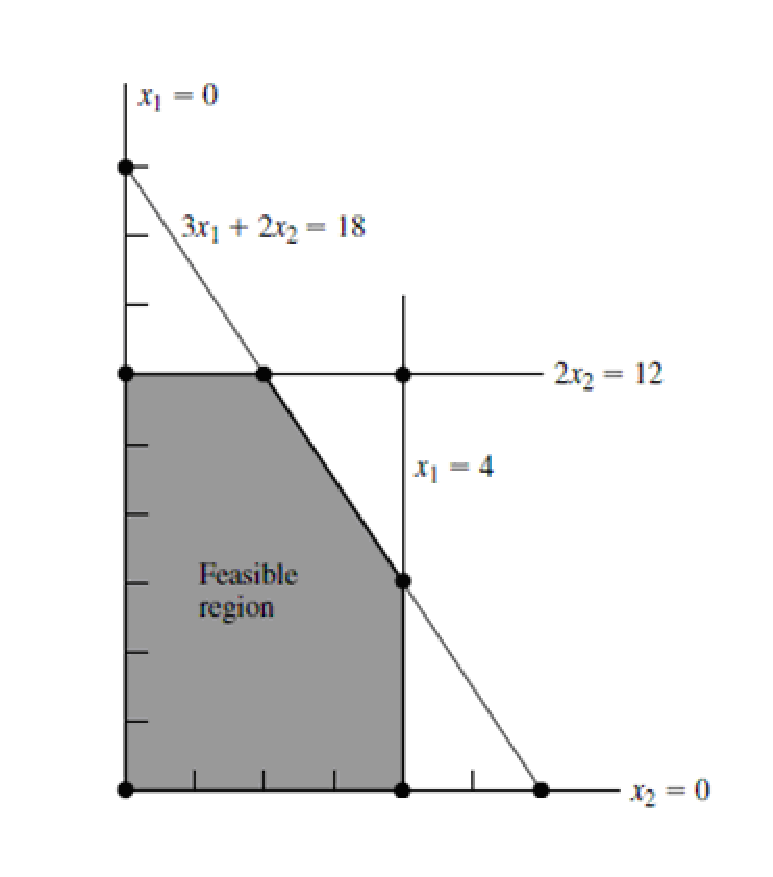
\includegraphics[scale=1.00]{graficos/simplex_grafico}
	\captionof{figure}{Representação gráfica de um Problema de Programação Linear de duas variáveis}
\end{center}

Onde cada reta representa uma restrição do modelo, e a área cinza representa a região viável, ou seja nessa área estão contidas os valores ótimos de $x_{1}$ e $x_{2}$ para a maximização do lucro.

Os método para resolução problemas de programação linear buscam a esse valores de $x_{1}$ e $x_{2}$  para determinação da solução ótima.

\section{Métodos de Solução}
Entre os métodos mais famosos para a resolução de problemas de programação linear estão o método simplex  e o método de pontos interiores. 
Depois da apresentação do método simplex,outros métodos com diferentes abordagens foram propostos \cite{Todd}. Porém, dentre os métodos existentes apenas o método de pontos interiores é atualmente competitivo em relação ao método simplex \apud{Bixby}{Munari}. 
A principal diferença entre esse dois métodos é o que o método simplex caminha pelos vértices da região viável, enquanto o método de pontos interiores caminha pelo interior da região viável \cite{MaculanPI}. Além disso, uma outra diferença é que o simplex exige muitas iterações com cálculos simples, enquanto o método de pontos interiores poucas iterações são exigidas, porém com cálculos mais elaborados.
Apesar das vantagens do método de pontos interiores em relação ao método estudado neste trabalho, o método simplex possui melhor desempenho na resolução de problemas de pequeno porte em relação ao método de pontos interiores, tornando-se um método indispensável em ferramentas de programação linear.

\subsection{Método Simplex}
O método simplex é um dos algoritmos mais populares para a resolução de problemas de programação linear. Surgiu a mais de 60 anos atrás e foi proposto por George Dantzig.  

É um método iterativo, e sua ideia principal consiste no fato de que a cada iteração uma nova solução é encontrada, sempre melhor que a anterior até o ponto em que a solução ótima é obtida. Outra característica do método é o fato de ser matricial, ou seja, os dados a serem calculados são armazenados em matrizes.  

Com a utilização do método foi percebido que a cada iteração do método simplex eram requeridos muitos cálculos sobre valores que nem sempre importavam para a iteração seguinte, fato que do ponto de vista computacional tornaria o método ineficiente.A partir desse fato foi desenvolvido o método simplex revisado visando a resolução de problemas de programação linear computacionalmente.

O presente trabalho tem foco no método simplex revisado e suas variantes.

\subsection{Método de Pontos Interiores}
Em 1984, Karmarkar revolucionou a área de programação linear com a publicação de um algoritmo de complexidade polinomial que apresentou bom desempenho quando aplicado a problemas práticos \cite{MaculanPI}. Essa publicação deu origem a um novo campo de pesquisa, chamado de método dos pontos interiores. 

O método de pontos interiores tem como principal característica a de realizar a busca por soluções no interior da região viável do problema, até encontrar a solução ótima \cite{Pinto}.
Em teoria, o método de pontos interiores é melhor que o método simplex, principalmente quando se leva em conta o critério de complexidade de pior caso. No entanto, na prática ambos os métodos concorrem até hoje. Já que o sucesso do método depende da estrutura dos problemas, da esparsidade \footnote{Quando uma matriz possui uma grande proporção de elementos nulos diz-se que é uma matriz esparsa \cite{Munari}.} e da arquitetura dos computadores \cite{MaculanPI}.

\section{Aplicações Práticas}
Um problema de programação linear, como já dito anteriormente, busca a otimização na distribuição de recursos sujeitos a restrições. Por isso é considerada uma poderosa ferramenta de apoio a decisão \cite{FrossardMaxMin} e com utilização em diversas áreas, como: indústria, saúde, computação, produção, etc.
As empresas, por exemplo, devem estar constantemente atentas a competitividade e as restrições existentes com o objetivo de alcançar suas metas, para isso é necessário otimizar os recursos disponíveis \cite{FrossardMaxMin}. Daí a importância da utilização da programação linear empregada em seu exemplo mais geral: maximizar o lucro e minimizar custos.  Na definição de modelos desse tipo deve-se considerar o preço de venda e o custo de produção, além de restrições do tipo: quantidade de matéria- prima e mão-de-obra disponíveis, máquinas disponíveis para produção, entre outros \cite{FrossardMaxMin}.
\begin{citacao}
“Administrar com eficiência os recursos disponíveis na empresa, através do planejamento, controle e execução das atividades relacionadas á utilização destes, é fator fundamental na busca da otimização do resultado global da empresa. A programação linear juntamente com as técnicas de pesquisa operacional, permite identificar o resultado ótimo, considerando todas as restrições impostas no modelo adotado.” \cite[p.~31]{FrossardMaxMin}
\end{citacao}

Outros exemplos bastante realistas da utilização da programação linear são os problemas de mistura e os de planejamento de produção e controle de estoque. No primeiro, basicamente trata-se da mistura de diferentes matérias para a produção de produtos, que devem obedecer a algumas especificações e, ao mesmo tempo, minimizar o custo ou maximizar o lucro. Já os problemas de planejamento de produção e controle de estoque possuem inúmeras aplicações, desde a alocação de máquinas para atender determinada demanda, até a utilização do estoque para atender a uma mudança imprevisível na demanda e necessidades de contratação de demissão para enfrentar mudanças nas necessidades de mão de obra \cite{Taha}.
A programação linear além de estar presente, é fundamental em diversas áreas, tornando-se uma ferramenta de apoio a decisão e contribuindo para o sucesso de projetos nas áreas em que se aplica.

\section{Ferramentas de Programação Linear}
Durante a pesquisa foram utilizadas e encontradas algumas ferramentas para a resolução de problemas de programação linear, além de bibliotecas com problemas testes. 
Uma das ferramentas é o Tora \cite{Taha}, que é software com uma interface simples, mas com algumas características que não há tornam muito amigável, além disso é um software mais educacional, inclusive com o recurso que mostra o passo a passo na resolução do problema utilizando o método simplex tabular.

\begin{center}
	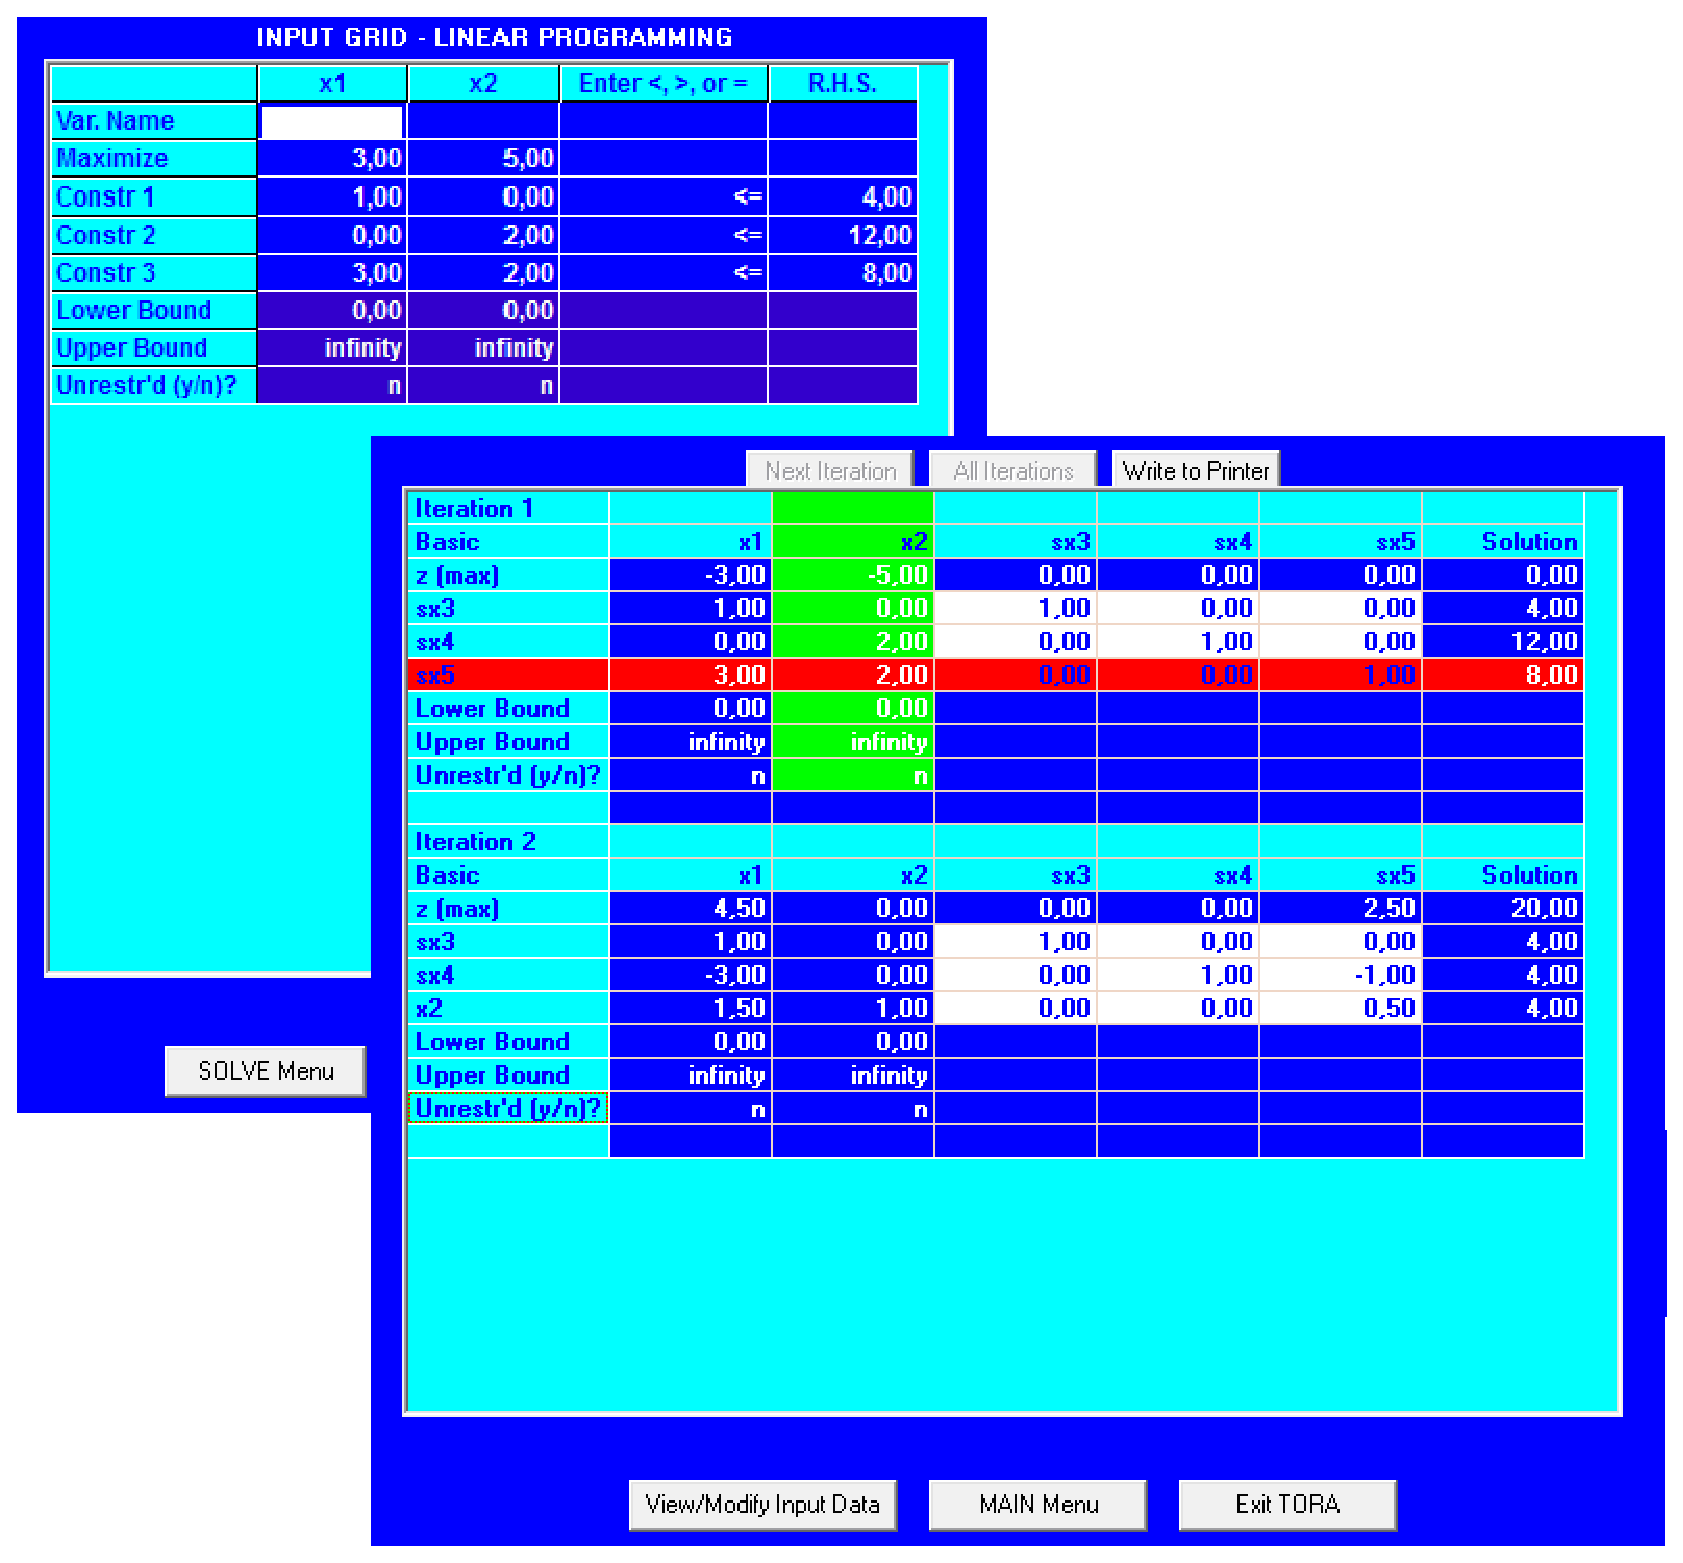
\includegraphics[scale=1.00]{tora}
	\captionof{figure}{Telas de entrada e sáida de dados do software Tora}
\end{center}

Já o Lingo disponibiliza uma versão demo gratuita. A maior dificuldade na utilização dessa ferramenta é o fato do usuário precisar digitar o modelo sem nenhuma orientação em relação a sintaxe, além disso a forma como o resultado é exibido dificulta a interpretação.
O Cplex é uma ferramenta mais robusta, com mais recursos e uma interface mais elaborada. Não é gratuita, mas uma versão com licença acadêmica é disponibilizada. Permite a modelagem e resolução de problemas de otimização de diversa natureza, como por exemplo: programação inteira, programação linear e programação inteira mista. Utilizando para isso diferentes métodos de solução.
O Glpk é um conjunto de rotinas destinadas a resolução de problemas de programação linear, além de problemas de programação inteira mista. As rotinas são escritas em ANSI C e podem ser utilizadas como biblioteca.
